\documentclass[10pt,journal,compsoc]{IEEEtran}

\usepackage{amsmath,amssymb,amsfonts,amsthm}
\usepackage{algorithmic}
\usepackage{algorithm}
\usepackage{graphicx}
\usepackage{textcomp}
\usepackage{xcolor}
\usepackage{booktabs}
\usepackage{cite}
\usepackage{url}
\usepackage{microtype}
\usepackage{subcaption}

\graphicspath{{../experiments/plots/}}

\newtheorem{theorem}{Theorem}
\newtheorem{lemma}{Lemma}
\newtheorem{proposition}{Proposition}
\newtheorem{definition}{Definition}
\newtheorem{corollary}{Corollary}

\begin{document}

\title{Cross-Flow Head-of-Line Blocking in Wi-Fi 7 Multi-Link Operation: Analytical Modeling and Sequence-Aware Scheduling}

\author{Research~Engineering~Group%
\thanks{Manuscript prepared for journal submission, October 2026. Complete source code, discrete-event simulation engine, experimental datasets across 30 paired random seeds, and automated test suites are preserved in the project artifact repository.}
}

\IEEEtitleabstractindextext{%
\begin{abstract}
The IEEE 802.11be (Wi-Fi 7) amendment introduces Multi-Link Operation (MLO) to aggregate throughput and reduce latency across multiple radio bands (2.4~GHz, 5~GHz, and 6~GHz). However, under standard multi-link Block Acknowledgment (BA) agreements, all application flows mapped to a common Traffic Identifier (TID) share a single, unified 12-bit sequence-number space and a common receiver reordering buffer. When heterogeneous frames are dispatched across parallel radio links with asymmetric transmission delays, contention backoffs, and frame error rates, out-of-order physical arrivals create severe Head-of-Line (HOL) reordering stalls. Crucially, a delayed frame from a bulk background flow traps subsequently-sequenced frames from latency-critical flows in the receiver buffer---a phenomenon we define as \emph{Cross-Flow Head-of-Line (CF-HOL) Blocking}.

In this paper, we develop a formal analytical framework and sender-side scheduling policy for CF-HOL blocking under standard IEEE 802.11be receiver semantics. First, we prove an orthogonal decomposition theorem demonstrating that total receiver reorder delay partitions additively and uniquely into intra-flow self-blocking and inter-flow cross-blocking ($\Delta_i = \mathcal{S}_i + \mathcal{X}_i$) as an exact trace accounting identity. Second, we establish the Multi-Link Sequence Divergence model, characterizing the mean-drift crossover boundary $\lambda^* = W / \delta$, deriving the exact Poisson stall probability $\Pr(N \ge W) = \gamma(W, \lambda_2 \delta) / (W-1)!$, and showing that approaching the boundary induces severe sliding window stalls with cumulative delay scaling as $\frac{1}{2} \lambda_2 \delta^2$. Third, we formulate the pairwise sequence assignment problem, proving that the optimal causal sequence order between concurrent candidate frames is uniquely determined by a transcendental threshold root $u^*(w_a, w_b)$ solved via Newton-Raphson iteration. We demonstrate that while this rule is provably optimal for pairs ($N=2$), transitivity fails for $N \ge 3$ candidate sets (generating Condorcet-style preference cycles), establishing multi-frame sequencing as an index heuristic. Fourth, we establish a symmetric-link causal uncertainty floor ($\min(w_a, w_b) \frac{\sigma_Z}{\sqrt{2\pi}}$) demonstrating that concurrent multi-link dispatch over stochastic Gaussian channels cannot achieve zero cross-flow delay. Guided by these results, we define \emph{Sequence-Aware Stochastic Partitioning (SASP)}, a transmitter-side policy that chooses the order in which queued frames of different flows receive sequence numbers, using causal estimates of per-link completion time; a Mean-Only variant omits the variance-aware pairwise threshold. We evaluate it in two independent simulators and report them separately. A custom Python discrete-event simulator (historical, 30 seeds) suggested cross-flow blocking reductions under link asymmetry, but these did not transfer: in a pinned ns-3.47 STR-MLO model, with a documented two-hook source patch placing the policy at the MAC's sequence-number commit point and a preregistered 810-run grid (three asymmetry levels, three loads, 30 seeds), the preregistered primary endpoint---mean cross-flow reorder wait of latency-sensitive packets under strong asymmetry and high load---was not reduced (paired difference $+0.0005$~ms, 95\% CI $[-0.0064,+0.0075]$~ms, $p=0.88$). What did change in ns-3 is latency-sensitive tail delay: the 99th-percentile delay fell by up to 17.5\% (Holm-adjusted $p<10^{-3}$ in seven of nine cells) with unchanged throughput and no retries. In a separate 810-run ablation with near-equal link means, both predictive arms reduced cross-flow wait relative to FIFO (16--21\% for Mean-Only), and the pairwise threshold rule added a further 6--27\% over Mean-Only, but only when the priority weights differ; the gain did not depend on the link-variance regime, so it is attributable to priority weighting rather than to variance awareness. All results are simulation results; no commercial hardware, firmware or production MAC was evaluated.

\end{abstract}

\begin{IEEEkeywords}
Wi-Fi 7, IEEE 802.11be, Multi-Link Operation (MLO), Block Acknowledgment, Head-of-Line Blocking, Packet Reordering, Stochastic Scheduling, Upper MAC.
\end{IEEEkeywords}}

\maketitle
\IEEEdisplaynontitleabstractindextext
\IEEEpeerreviewmaketitle

\section{Introduction}
\label{sec:intro}

The IEEE 802.11be Extremely High Throughput (EHT) amendment, commercialized under the trade name Wi-Fi 7, establishes Multi-Link Operation (MLO) as its architectural cornerstone~\cite{ieee80211be2024}. By allowing affiliated Multi-Link Devices (MLDs) to coordinate transmissions across multiple physical interfaces operating simultaneously in the 2.4~GHz, 5~GHz, and 6~GHz bands, MLO delivers unprecedented multi-gigabit throughput and promises deterministic sub-millisecond latencies for emerging real-time applications such as cloud gaming, augmented reality (XR), and industrial robotics.

To manage parallel radio access without redesigning higher network layers, the IEEE 802.11be MAC architecture is divided into an Upper MAC (U-MAC) and multiple Lower MACs (L-MACs)~\cite{choi2025joint}. The U-MAC is responsible for queue management, multi-link packet scheduling, and flow-level coordination, whereas each L-MAC manages link-specific physical carrier sensing, Enhanced Distributed Channel Access (EDCA) backoff, and Physical Layer Convergence Protocol (PLCP) encapsulation.

Under the 802.11be specification, the Block Acknowledgment (BA) mechanism operates at the U-MAC level per peer MLD and Traffic Identifier ($\text{TID} \in \{0, \dots, 7\}$)~\cite{ieee80211be2024}:
\begin{enumerate}
    \item A single, unified 12-bit sequence-number space ($s \in [0, 4095]$) is shared by all MAC Service Data Units (MSDUs) transmitted under a given TID across all active links.
    \item The receiver MLD maintains a single sliding receive reordering buffer governed by window size $W \in \{64, 256, 1024\}$ and window base $W_{\text{start}}$.
    \item The receiver delivers MSDUs to the upper layers (Logical Link Control/IP) strictly in monotonically increasing sequence-number order.
\end{enumerate}

While this unified sequence space guarantees backward compatibility with legacy 802.11 state machines and prevents out-of-order segment delivery to transport protocols like TCP, it creates an acute performance vulnerability when links exhibit heterogeneous physical channel characteristics~\cite{carreno2021multi,oliveira2026characterizing}. In modern wireless environments, parallel links inevitably differ in bandwidth (e.g., 20~MHz on 2.4~GHz vs. 160/320~MHz on 5/6~GHz), PHY data rates, channel contention (EDCA contention slot delays), and Frame Error Rates (FER).

When sequence numbers are assigned conventionally in arrival order (FIFO), an earlier-sequenced frame dispatched over a slower, congested, or lossy link will complete physical transmission significantly later than subsequently-sequenced frames dispatched over a clear, high-speed link. Consequently, successfully received frames are trapped inside the receiver reordering buffer awaiting the missing earlier sequence number.

This bottleneck becomes critical when heterogeneous application flows share the same TID. Because the IEEE 802.11 standard defines only eight TIDs mapped to four Access Categories (AC\_VO, AC\_VI, AC\_BE, AC\_BK), host operating systems routinely multiplex diverse application flows---such as interactive VoIP, cloud gaming telemetry, and bulk background file synchronization---into the default Best Effort Access Category (TID 0)~\cite{carreno2021multi,sangeetha2026performance}. In such deployments:
\begin{itemize}
    \item A bulk packet dispatched on a slow 2.4~GHz link receives sequence number $s$.
    \item Latency-critical gaming packets dispatched on a 6~GHz link receive sequence numbers $s+1, s+2, \dots, s+k$.
    \item Although the gaming packets arrive physically in fractions of a millisecond, the receiver cannot deliver them to the host network stack until packet $s$ arrives or undergoes retries.
\end{itemize}
We formally define this phenomenon as \textbf{Cross-Flow Head-of-Line (CF-HOL) Blocking}.

Recent empirical measurements by Oliveira et al.~\cite{oliveira2026characterizing} in ns-3 confirmed that multi-link reordering causes severe latency degradation. However, existing work suffers from three decisive limitations:
\begin{enumerate}
    \item \emph{Absence of Mathematical Modeling:} Prior studies~\cite{oliveira2026characterizing,alhraishawi2022delay} treat multi-link reordering empirically without formalizing the stochastic coupling between channel completion variances and sliding BA window dynamics.
    \item \emph{Confounded Delay Metrics:} Existing literature measures only aggregate end-to-end latency, failing to mathematically decouple intra-flow self-reordering from inter-flow cross-blocking.
    \item \emph{Non-Standard or Receiver-Side Proposals:} Proprietary patents, such as MediaTek US12470496B2~\cite{mediatek2024reordering}, propose receiver-side Deep Packet Inspection (DPI) to construct per-flow reorder queues. This violates standard IEEE 802.11be protocol semantics, requires specialized receiver silicon, and leaves commercial off-the-shelf client devices completely unprotected.
\end{enumerate}

\textbf{Contributions:} In this paper, we resolve these challenges by establishing an analytical modeling framework and transmitter-side scheduling architecture for CF-HOL blocking in Wi-Fi 7:
\begin{itemize}
    \item \textbf{Orthogonal Delay Decomposition (Theorem 1):} We prove that total receiver reordering delay decomposes additively, uniquely, and non-negatively into intra-flow self-blocking and inter-flow cross-blocking ($\Delta_i = \mathcal{S}_i + \mathcal{X}_i$) as an exact post-facto trace accounting framework.
    \item \textbf{Sequence Divergence \& Stall Probability (Theorem 2):} We establish the mean-drift crossover boundary $\lambda^* = W / \delta$, derive the exact Poisson stall probability $\Pr(N \ge W) = \gamma(W, \lambda_2 \delta) / (W-1)!$, and prove quadratic cumulative stall scaling $\frac{1}{2} \lambda_2 \delta^2$.
    \item \textbf{Optimal Pairwise Predictive Sequencing Rule (Theorem 3):} We formulate the pairwise sequence assignment problem, proving that the optimal causal sequence order between concurrent candidate frames is uniquely determined by a transcendental threshold root $u^*(w_a, w_b)$ solved via Newton-Raphson in $\le 4$ steps. We formally establish that pairwise preferences fail transitivity for $N \ge 3$ frames (demonstrating strict Condorcet cycles), characterizing multi-frame sequencing as an index heuristic.
    \item \textbf{Symmetric-Link Uncertainty Floor (Theorem 4):} We prove that concurrent dispatch over symmetric stochastic links has an irreducible cross-flow delay floor $\min(w_a, w_b) \frac{\sigma_Z}{\sqrt{2\pi}}$, while explicitly identifying its boundaries (e.g., Single-Link Operation achieves $\mathcal{X}=0$).
    \item \textbf{The SASP Policy \& Two-Simulator Evaluation:} We define \emph{Sequence-Aware Stochastic Partitioning (SASP)}, a transmitter-side sequence-assignment policy, and evaluate it in a custom Python simulator (historical results, Section~\ref{sec:eval}) and in a pinned ns-3.47 STR-MLO model with a documented source patch (Section~\ref{sec:ns3}). The ns-3 study is preregistered, uses 30 seeds per cell, and reports a null result on the primary endpoint, a significant tail-delay improvement for latency-sensitive traffic, and an ablation showing that the pairwise threshold's incremental benefit tracks priority weighting rather than link variance.
\end{itemize}

\section{Related Work and Prior Art Context}
\label{sec:related}

\subsection{Multi-Link Operation in IEEE 802.11be}
The Multi-Link Operation (MLO) architecture defined in IEEE Std 802.11be-2024 provides two primary operational modes: Simultaneous Transmit and Receive (STR) and Non-Simultaneous Transmit and Receive (NSTR)~\cite{ieee80211be2024}. In STR mode, an MLD can transmit or receive simultaneously on multiple links without cross-band in-device interference (e.g., between 5~GHz and 6~GHz). Carre{\~n}o et al.~\cite{carreno2021multi} conducted early throughput studies of MLO, observing that when links exhibit severe rate asymmetry, naive multi-link aggregation can paradoxically degrade overall performance compared to single-link operation. Levy et al.~\cite{levy2022mlo} and Al-Hraishawi et al.~\cite{alhraishawi2022delay} analyzed MLO delay under finite queue loads, but both studies assumed single-flow Poisson arrivals and ideal in-order reception.

\subsection{Reorder Buffering and Block Acknowledgment Dynamics}
The Block Acknowledgment (BA) mechanism originated in IEEE 802.11e and was extended in 802.11n/ac/ax for high-speed frame aggregation (A-MPDU). In 802.11be MLO, the BA agreement operates at the peer MLD level across all links affiliated with a TID~\cite{ieee80211be2024}. 

Oliveira, Raposo, and Lu{\'{i}}s (2026)~\cite{oliveira2026characterizing} characterized out-of-order delivery and Block Ack buffer waiting under Wi-Fi 7 MLO using ns-3; BA-window reordering in MLO is therefore an established problem, and the question here is narrower: whether a transmitter-side sequence-assignment policy can reduce the \emph{cross-flow} part of that waiting when flows share a TID. Sangeetha et al.~\cite{sangeetha2026performance} presented an analytical model for unsaturated MLO queues using a multi-dimensional Markov chain, but their formulation assumed that each traffic flow possesses a dedicated TID, sidestepping single-TID multi-flow contention. Choi, Jung, and Kim~\cite{choi2025joint} studied joint L-MAC transmission and U-MAC packet scheduling for NSTR MLO with an in-house simulator; their focus is packet-to-link scheduling in the NSTR setting. ATLAS~\cite{atlas2026} proposes adaptive traffic-to-link allocation to reduce delay, accounting for expected access and queueing delay and U-MAC holding delay. Traffic-to-link allocation and latency-aware U-MAC scheduling are thus established topics; SASP does not allocate flows to links and is distinguished only by acting on the order of sequence-number assignment within a shared TID.

\subsection{Multipath Transport Schedulers vs. Wireless MAC}
Out-of-order packet reordering has been extensively studied at the transport layer, particularly in Multipath TCP (MPTCP)~\cite{ferlin2016blest}. Schedulers such as BLEST (Blocking Estimation-based MPTCP Scheduler)~\cite{ferlin2016blest} predict head-of-line receiver blocking by comparing estimated path Round-Trip Times (RTTs). 

However, transport-layer schedulers operate on continuous byte streams over long RTT timescales (10--100~ms) with explicit end-to-end ACK feedback. In contrast, wireless Upper MAC scheduling operates on discrete frames at sub-millisecond timescales ($100\,\mu\text{s}$--$5\,\text{ms}$) under non-stationary EDCA contention backoff, small sliding sequence windows ($W \in \{64, 256\}$), and rapid burst fading. Consequently, MPTCP heuristics cannot be directly applied to the 802.11be U-MAC.

\subsection{Architectural Boundary and Patent Landscape}
To mitigate MLO reordering stalls, proprietary patent filings have emerged. Most notably, MediaTek patent US12470496B2~\cite{mediatek2024reordering} proposes a \emph{receiving apparatus} that performs Deep Packet Inspection (DPI) on incoming MPDUs, inspects IP/UDP 5-tuple headers, and demultiplexes packets into separate per-flow receive queues before releasing them to upper layers.

While effective in closed ecosystems, this approach has severe practical drawbacks:
\begin{enumerate}
    \item It alters standard IEEE 802.11be receiver protocol semantics, which dictate a single TID reordering buffer.
    \item It cannot accelerate standard commercial client stations (smartphones, IoT devices) that implement unmodified 802.11be MAC firmware.
    \item It requires packet header inspection hardware on power-constrained mobile receivers.
\end{enumerate}
In contrast, our proposed SASP algorithm resides \textbf{strictly at the transmitting U-MAC}. The transmitter optimizes link dispatch and sequence numbering such that packets arrive physically in sequential order at the receiver. Standard commercial client devices receive packets within valid sequence windows and deliver them with zero stalls, guaranteeing full protocol compliance and complete independence from receiver-side patents. (We note that this comparison represents an engineering prior-art analysis and does not constitute a formal legal freedom-to-operate opinion.)

\section{System Model and Problem Formulation}
\label{sec:system_model}

\subsection{Multi-Link MAC Sublayer Architecture}
We consider an IEEE 802.11be Access Point (AP) MLD communicating with an affiliated non-AP station MLD over a set of $K \ge 2$ orthogonal radio links $\mathcal{K} = \{1, 2, \dots, K\}$. We assume Simultaneous Transmit and Receive (STR) operation across non-overlapping frequency bands (Link 1: 2.4~GHz, Link 2: 5~GHz, Link 3: 6~GHz).

A set of $M \ge 2$ distinct application flows $\mathcal{F} = \{1, \dots, M\}$ generate packets mapped to a single TID (e.g., TID 0, Best Effort). Each flow $f \in \mathcal{F}$ is characterized by an arrival rate $\lambda_f$ and a delay penalty weight $w_f > 0$. Higher weights denote latency-sensitive traffic (e.g., $w_{\text{gaming}} = 20, w_{\text{bulk}} = 1$). Incoming packets are queued in flow-specific U-MAC buffers $Q_1, \dots, Q_M$.

\subsection{Lower MAC Channel Access and Service Times}
Each radio link $k \in \mathcal{K}$ executes an independent EDCA channel access engine with parameters $(\text{AIFS}_k, \text{CW}_{\min, k}, \text{CW}_{\max, k})$ and PHY transmission rate $R_k$. When packet $i$ of length $L_i$ bits is dispatched to link $\ell_i = k$ at dispatch time $t_i^{\text{disp}}$, its total completion duration until successful Block Ack confirmation is:
\begin{equation}
    D_i(k) = \sum_{r=1}^{N_{i, k}} \left( B_{k, r} + T_{\text{frame}, k}(L_i) \right) + T_{\text{ack}, k}
\end{equation}
where $N_{i, k} \in [1, N_{\max}]$ is the number of transmission attempts until success, $B_{k, r}$ is the stochastic EDCA backoff slot duration, $T_{\text{frame}, k}$ is the PLCP frame transmission time, and $T_{\text{ack}, k}$ is the turnaround and Block Ack response time. The physical arrival time of packet $i$ at the receiver is:
\begin{equation}
    A_i = t_i^{\text{disp}} + D_i(\ell_i)
\end{equation}
The link service duration $D_i(k)$ is modeled as a continuous random variable with mean $\mu_k$ and variance $\sigma_k^2$. Channel error dynamics are captured via a two-state Gilbert-Elliott model alternating between Good and Bad channel states.

\begin{table*}[t]
\centering
\caption{System Model and Simulation Parameters}
\label{tab:params}
\begin{tabular}{lccc}
\toprule
\textbf{Parameter} & \textbf{Link 1 (2.4 GHz)} & \textbf{Link 2 (5 GHz)} & \textbf{Link 3 (6 GHz)} \\
\midrule
Channel Width & 20 MHz & 80 MHz & 160 MHz \\
Base MCS & MCS 4 & MCS 9 & MCS 11 \\
PHY Rate ($R_k$) & 39.0 Mbps & 480.4 Mbps & 1201.0 Mbps \\
AIFS & 3 slots & 2 slots & 2 slots \\
$\text{CW}_{\min} / \text{CW}_{\max}$ & 15 / 1023 & 15 / 1023 & 15 / 1023 \\
Slot Time & $9\,\mu\text{s}$ & $9\,\mu\text{s}$ & $9\,\mu\text{s}$ \\
Base Delay ($\mu_k$) & 1.20 ms & 0.40 ms & 0.25 ms \\
Jitter ($\sigma_k$) & 0.35 ms & 0.12 ms & 0.08 ms \\
Frame Error Rate & $0.05 - 0.15$ & $0.02 - 0.08$ & $0.01 - 0.05$ \\
\bottomrule
\end{tabular}
\end{table*}

\subsection{Receiver Block Ack Reorder Buffer}
The receiver MLD manages a single reordering buffer of size $W \in \{64, 256, 1024\}$ for the given TID. The active sequence window is $[W_{\text{start}}, W_{\text{start}} + W - 1]$. Upon physical arrival of packet $i$ at time $A_i$ with sequence number $s_i$:
\begin{itemize}
    \item If $s_i = W_{\text{start}}$: Packet $i$ is immediately delivered to upper layers, and $W_{\text{start}}$ advances to the lowest missing sequence number.
    \item If $W_{\text{start}} < s_i < W_{\text{start}} + W$: Packet $i$ is retained in the buffer awaiting all missing predecessors $\{s' : W_{\text{start}} \le s' < s_i\}$.
    \item If $s_i \ge W_{\text{start}} + W$: The buffer window overflows. To prevent indefinite stalls, $W_{\text{start}}$ is forcefully advanced to $s_i - W + 1$, and all missing packets prior to the new $W_{\text{start}}$ are declared lost.
\end{itemize}
Under reliable transmission, packet $i$ is released to the host stack at time:
\begin{equation}
    R_i = \max\left(A_i, \max_{k: s_k < s_i} A_k\right)
\end{equation}
The total reordering delay experienced by packet $i$ is $\Delta_i = R_i - A_i \ge 0$.

\section{Theoretical Analysis and Theorems}
\label{sec:theory}

\subsection{Orthogonal Delay Decomposition}

To rigorously study multi-flow interference, we must isolate the delay intrinsic to a flow's own dispersion from the delay imposed by competing flows sharing the TID.

\begin{theorem}[Buffer Reorder Accounting Decomposition]
\label{thm:decomp}
Let packet $i$ belong to flow $f_i$ with physical arrival time $A_i$ and assigned sequence number $s_i$. On an observed execution trace, define the intra-flow completion boundary:
\begin{equation}
    R_i^{\text{intra}} \triangleq \max\left(A_i, \max_{j: f_j = f_i, s_j < s_i} A_j\right)
\end{equation}
Then the total reordering delay $\Delta_i = R_i - A_i$ admits an exact, non-negative, additive decomposition:
\begin{equation}
    \Delta_i = \mathcal{S}_i + \mathcal{X}_i
\end{equation}
where:
\begin{equation}
    \mathcal{S}_i \triangleq R_i^{\text{intra}} - A_i = \max\left(0, \max_{j: f_j = f_i, s_j < s_i} A_j - A_i\right)
\end{equation}
denotes the intra-flow \textbf{Self-Blocking Delay}, and:
\begin{equation}
    \mathcal{X}_i \triangleq R_i - R_i^{\text{intra}} = \max\left(0, \max_{k: f_k \ne f_i, s_k < s_i} A_k - R_i^{\text{intra}}\right)
\end{equation}
denotes the inter-flow \textbf{Cross-Flow Blocking Delay}.
\end{theorem}

\begin{proof}
By IEEE 802.11be in-order delivery semantics, the delivery epoch is $R_i = \max(A_i, \max_{k: s_k < s_i} A_k)$. The set of causal predecessors $\mathcal{P}_i = \{k : s_k < s_i\}$ partitions into disjoint intra-flow predecessors $\mathcal{P}_i^{\text{intra}} = \{j : f_j = f_i, s_j < s_i\}$ and inter-flow predecessors $\mathcal{P}_i^{\text{inter}} = \{k : f_k \ne f_i, s_k < s_i\}$. Hence:
\begin{equation}
    R_i = \max\left( R_i^{\text{intra}}, \max_{k \in \mathcal{P}_i^{\text{inter}}} A_k \right)
\end{equation}
Since $R_i \ge R_i^{\text{intra}} \ge A_i$, both $\mathcal{S}_i \ge 0$ and $\mathcal{X}_i \ge 0$. Summing:
\begin{equation}
    \mathcal{S}_i + \mathcal{X}_i = (R_i^{\text{intra}} - A_i) + (R_i - R_i^{\text{intra}}) = R_i - A_i = \Delta_i
\end{equation}
\end{proof}

\begin{lemma}[Attribution Invariance and Boundary Conditions]
\label{lem:invariance}
On an observed trace with fixed physical arrival epochs $\{A_i\}$ and sequence numbers $\{s_i\}$, the self-blocking delay $\mathcal{S}_i$ is strictly invariant to the arrival epochs, sequence numbers, and presence of all competing flows $\mathcal{F} \setminus \{f_i\}$. 

\emph{Physical Boundary Note:} This invariance is an in-buffer accounting property on a realized trace. In a real shared wireless medium, the physical presence of competing traffic introduces EDCA channel contention, collision-induced backoff escalation, and queuing delay, which dynamically alters $\{A_i\}$. Theorem~\ref{thm:decomp} thus serves as an exact diagnostic metric for isolating in-buffer reordering stalls from channel service time dispersion.
\end{lemma}
\begin{proof}
By definition, $R_i^{\text{intra}}$ depends exclusively on $A_i$ and the set $\{A_j : f_j = f_i, s_j < s_i\}$. Removing all frames of other flows leaves $\mathcal{P}_i^{\text{inter}} = \emptyset$, which forces $R_i = R_i^{\text{intra}}$ and $\mathcal{X}_i = 0$, while $\mathcal{S}_i$ remains unchanged.
\end{proof}

\subsection{Multi-Link Sequence Divergence and Buffer Stability}

We now analyze the stochastic behavior of the receiver sliding window when flows with asymmetric rates and delays share a TID under standard FIFO sequence assignment.

\begin{theorem}[Sequence Divergence and Buffer Stall Probability]
\label{thm:collapse}
Consider an MLD transmitting bulk flow $A$ on slow Link 1 ($\mu_1, \sigma_1^2$) and interactive flow $B$ on fast Link 2 ($\mu_2, \sigma_2^2$) with mean asymmetry $\delta = \mu_1 - \mu_2 > 0$ and negotiated Block Ack window $W$. Under FIFO sequencing:
\begin{enumerate}
    \item During the completion duration of a frame on Link 1, the sequence divergence $N$ on Link 2 has mean $\mathbb{E}[N] = \lambda_B \mu_1$. Under Poisson arrivals, $\operatorname{Var}(N) = \lambda_B \mu_1 + \lambda_B^2 \sigma_1^2$.
    \item The mean-drift crossover boundary occurs at critical arrival rate:
    \begin{equation}
        \lambda^* \triangleq \frac{W}{\delta}
    \end{equation}
    When $\lambda_B > \lambda^*$, the mean queue drift into the reorder window is positive ($\mathbb{E}[N] > W$), causing buffer accumulation on average.
    \item For constant completion duration $\delta$ on Link 1 and Poisson arrivals at rate $\lambda_B$ on Link 2, the exact probability that the sequence gap reaches or exceeds window capacity $W$ is:
    \begin{align}
        P_{\text{stall}}(\lambda_B, \delta, W) &\triangleq \Pr(N \ge W) \nonumber \\
        &= 1 - \sum_{k=0}^{W-1} \frac{(\lambda_B \delta)^k e^{-\lambda_B \delta}}{k!} \nonumber \\
        &= \frac{\gamma(W, \lambda_B \delta)}{(W-1)!}
    \end{align}
    For any finite $\lambda_B$, $\Pr(N < W) > 0$. At $\lambda_B = \lambda^*$, $P_{\text{stall}} \approx 0.533$ for $W=16$, with $P(N < W) \approx 0.467$.
    \item The cumulative cross-flow blocking duration per frame of flow $A$ scales quadratically as:
    \begin{equation}
        \int_0^{\lambda_B \delta} \left(\delta - \frac{x}{\lambda_B}\right) dx = \frac{1}{2} \lambda_B \delta^2
    \end{equation}
\end{enumerate}
\end{theorem}

\begin{proof}
Frame $a$ of flow $A$ is dispatched to Link 1 at $t=0$, completing at $D_1$ with $\mathbb{E}[D_1] = \mu_1$. Concurrently, frames $b_j$ ($j = 1, 2, \dots$) are dispatched on Link 2 at rate $\lambda_B$ with sequence numbers $s_j = s_a + j$. Frame $b_j$ completes at $A_{b_j} = j / \lambda_B + D_{2, j}$. Whenever $j / \lambda_B + D_{2, j} < D_1$, packet $b_j$ arrives before frame $a$ and is cross-blocked: $\mathcal{X}_{b_j} = \delta - j / \lambda_B$. Integrating across $j \in [0, \lambda_B \delta]$:
\begin{equation}
    \int_0^{\lambda_B \delta} \left(\delta - \frac{x}{\lambda_B}\right) dx = \lambda_B \delta^2 - \frac{\lambda_B^2 \delta^2}{2\lambda_B} = \frac{1}{2} \lambda_B \delta^2
\end{equation}
By the law of total expectation and variance for compounded Poisson arrivals: $\mathbb{E}[N] = \lambda_B \mu_1$, $\operatorname{Var}(N) = \lambda_B \mu_1 + \lambda_B^2 \sigma_1^2$. The complement probability of reaching or exceeding window capacity follows directly from the Poisson cumulative distribution function.
\end{proof}

\subsection{Optimal Predictive Sequencing Rule (SASP)}

We now address the core scheduling problem: given candidate frames ready for transmission across parallel links, how should sequence numbers be assigned to minimize total weighted cross-flow blocking?

\begin{theorem}[SASP Optimal Pairwise Threshold Rule]
\label{thm:sasp}
Let candidate frames $a$ (flow $f_a$, weight $w_a$) and $b$ (flow $f_b$, weight $w_b$, $f_a \ne f_b$) have completion times $A_a \sim \mathcal{N}(\mu_a, \sigma_a^2)$ and $A_b \sim \mathcal{N}(\mu_b, \sigma_b^2)$. Let $Z \triangleq A_a - A_b \sim \mathcal{N}(\mu_Z, \sigma_Z^2)$, with $\mu_Z = \mu_a - \mu_b$ and $\sigma_Z = \sqrt{\sigma_a^2 + \sigma_b^2}$.

The sequence assignment decision minimizing expected weighted cross-flow blocking cost:
\begin{align}
    C(s_a < s_b) &= w_b \mathbb{E}[(A_a - A_b)^+], \nonumber \\
    C(s_b < s_a) &= w_a \mathbb{E}[(A_b - A_a)^+]
\end{align}
is given by the strictly optimal pairwise threshold rule:
\begin{equation}
    s_a < s_b \iff \frac{\mu_a - \mu_b}{\sqrt{\sigma_a^2 + \sigma_b^2}} \le u^*(w_a, w_b)
\end{equation}
where $u^*$ is the unique root of the strictly monotonically increasing function:
\begin{equation}
    h(u) \triangleq (w_b - w_a) \phi(u) + \left[ w_a(1 - \Phi(u)) + w_b\Phi(u) \right] u = 0
\end{equation}
and $\phi(\cdot)$, $\Phi(\cdot)$ are the standard Gaussian PDF and CDF.

Properties of the Root $u^*$:
\begin{enumerate}
    \item When flow weights are equal ($w_a = w_b$), $u^* = 0$, and optimal sequence assignment is sorted strictly by expected completion time: $s_a < s_b \iff \mu_a \le \mu_b$.
    \item When flow $b$ has higher priority ($w_b > w_a$), $u^* < 0$, satisfying $|u^*| \le \sqrt{2 \ln(w_b / w_a)}$.
    \item $u^*$ is transcendental and computed via Newton-Raphson iteration in $\le 4$ steps.
    \item \textbf{Non-Transitivity for $N \ge 3$ Frames:} For $N \ge 3$ candidates, the pairwise preference relation $a \prec b \iff C(s_a < s_b) \le C(s_b < s_a)$ is non-transitive in general (exhibiting Condorcet-style preference cycles $A \prec B \prec C \prec A$). Thus, greedy pairwise sorting is an index heuristic, not a globally optimal batch policy.
\end{enumerate}
\end{theorem}

\begin{proof}
Using the identity $Z^+ - (-Z)^+ = Z$, we have $\mathbb{E}[(-Z)^+] = \mathbb{E}[Z^+] - \mu_Z$. The condition $C(s_a < s_b) \le C(s_b < s_a)$ is equivalent to $(w_b - w_a) \mathbb{E}[Z^+] + w_a \mu_Z \le 0$. For $Z \sim \mathcal{N}(\mu_Z, \sigma_Z^2)$, normalized variable $u = \mu_Z / \sigma_Z$. Truncated normal expectation yields:
\begin{equation}
    \mathbb{E}[Z^+] = \sigma_Z \left[ \phi(u) + u \Phi(u) \right]
\end{equation}
Dividing by $\sigma_Z > 0$ yields:
\begin{equation}
    (w_b - w_a)\phi(u) + \left[w_a(1-\Phi(u)) + w_b\Phi(u)\right]u \le 0
\end{equation}
Taking the first derivative of $h(u)$ with respect to $u$:
\begin{align}
    h'(u) &= (w_b - w_a)(-u\phi(u)) + (w_b - w_a)(u\phi(u)) \nonumber \\
    &\quad + \left[ w_a(1-\Phi(u)) + w_b\Phi(u) \right]
\end{align}
The first two terms cancel identically! Hence:
\begin{equation}
    h'(u) = w_a (1 - \Phi(u)) + w_b \Phi(u) > 0, \quad \forall u \in \mathbb{R}
\end{equation}
Because $h'(u) > 0$ strictly everywhere, $h(u)$ is strictly monotonically increasing from $-\infty$ to $+\infty$. By the Intermediate Value Theorem, $h(u) = 0$ possesses exactly one real root $u^*$.
\end{proof}

\subsection{Symmetric-Link Causal Uncertainty Floor}

\begin{theorem}[Symmetric-Link Causal Uncertainty Floor]
\label{thm:lower_bound}
When candidate frames $a$ and $b$ are dispatched concurrently on stochastic links with equal mean completion times ($\mu_a = \mu_b$, so $u = 0$) and non-zero Gaussian variance $\sigma_Z = \sqrt{\sigma_a^2 + \sigma_b^2} > 0$, the expected weighted cross-flow blocking cost under any binary sequence assignment decision is strictly lower-bounded by:
\begin{equation}
    \min\left( C(s_a < s_b), C(s_b < s_a) \right) = \min(w_a, w_b) \frac{\sigma_Z}{\sqrt{2\pi}} > 0
\end{equation}
For arbitrary link asymmetry $u = (\mu_a - \mu_b) / \sigma_Z$, the optimal decision cost attains its global maximum at $u = u^*$ and decays to zero as $|u| \to \infty$.

\emph{Falsification Boundaries:} This bound holds strictly conditional on concurrent multi-link dispatch over stochastic channels. Under Single-Link Operation (SLO) or deterministic links ($\sigma_Z = 0$), frames arrive in sequential order, achieving $\mathcal{X}_i = 0$ identically.
\end{theorem}

\begin{proof}
At $u = 0$, $\phi(0) = \frac{1}{\sqrt{2\pi}}$, $\Phi(0) = \frac{1}{2}$, and $\mu_Z = 0$. Hence $\mathbb{E}[Z^+] = \mathbb{E}[(-Z)^+] = \sigma_Z \phi(0) = \frac{\sigma_Z}{\sqrt{2\pi}}$. Evaluating $C(s_a < s_b) = w_b \frac{\sigma_Z}{\sqrt{2\pi}}$ and $C(s_b < s_a) = w_a \frac{\sigma_Z}{\sqrt{2\pi}}$ gives $\min(C) = \min(w_a, w_b) \frac{\sigma_Z}{\sqrt{2\pi}}$. As $|u| \to \infty$, Mill's ratio ensures $C^*(u) \to 0$.
\end{proof}

\section{The SASP Scheduling Algorithm}
\label{sec:algorithm}

\subsection{Algorithmic Design}
Algorithm~\ref{alg:sasp} presents the complete specification of \emph{Sequence-Aware Stochastic Partitioning (SASP)}, implemented at the transmitter U-MAC.

\begin{algorithm}[t]
\caption{Sequence-Aware Stochastic Partitioning (SASP)}
\label{alg:sasp}
\begin{algorithmic}[1]
\REQUIRE Queues $\{Q_f\}_{f=1}^M$, Links $\mathcal{K}$, Window $W$, Flow weights $\{w_f\}$.
\ENSURE Dispatched tuple $(p^*, \ell^*, s^*)$.
\STATE $\text{Cost}_{\min} \leftarrow \infty, (p^*, \ell^*) \leftarrow \text{None}$
\FORALL{available link $\ell \in \mathcal{K}$}
    \STATE Read current estimates $(\hat{\mu}_\ell, \hat{\sigma}_\ell)$ from EWMA tracker.
    \FORALL{active flow $f \in \mathcal{F}$ with $Q_f \ne \emptyset$}
        \STATE $p \leftarrow Q_f.\text{peek}()$
        \STATE $\hat{A}_{\text{cand}} \leftarrow t_{\text{curr}} + \hat{\mu}_\ell$
        \STATE $\text{Cost} \leftarrow w_f \cdot \hat{\mu}_\ell$
        \FORALL{in-flight unacknowledged packet $p_j \in \mathcal{O}$ with $f_j \ne f$}
            \STATE $\Delta\mu \leftarrow \hat{A}_j - \hat{A}_{\text{cand}}$
            \STATE $\sigma_Z \leftarrow \sqrt{\hat{\sigma}_\ell^2 + \hat{\sigma}_j^2}$
            \STATE Compute $u^* \leftarrow \text{SolveRoot}(w_j, w_f)$ via Newton-Raphson.
            \IF{$\Delta\mu / \sigma_Z \ge u^*$}
                \STATE $\text{Cost} \mathrel{+}= w_f \cdot \sigma_Z \left[ \phi(\frac{\Delta\mu}{\sigma_Z}) + \frac{\Delta\mu}{\sigma_Z} \Phi(\frac{\Delta\mu}{\sigma_Z}) \right]$
            \ELSE
                \STATE $\text{Cost} \mathrel{+}= w_j \cdot \sigma_Z \left[ \phi(-\frac{\Delta\mu}{\sigma_Z}) - \frac{\Delta\mu}{\sigma_Z} \Phi(-\frac{\Delta\mu}{\sigma_Z}) \right]$
            \ENDIF
        \ENDFOR
        \IF{$\text{Cost} < \text{Cost}_{\min}$}
            \STATE $\text{Cost}_{\min} \leftarrow \text{Cost}, p^* \leftarrow p, \ell^* \leftarrow \ell$
        \ENDIF
    \ENDFOR
\ENDFOR
\STATE $p^* \leftarrow Q_{f^*}.\text{pop}()$
\STATE Assign $s^* \leftarrow \text{AllocateSequenceNumber}(p^*, \ell^*, W)$.
\STATE Dispatch $p^*$ to L-MAC on link $\ell^*$.
\end{algorithmic}
\end{algorithm}

\subsection{Parameter Estimation and Complexity}
Channel completion parameters $(\hat{\mu}_\ell, \hat{\sigma}_\ell^2)$ are updated at runtime upon receiving Block Ack frames using an Exponentially Weighted Moving Average (EWMA) with smoothing factor $\alpha = 0.125$. The threshold root $u^*$ converges in $\le 4$ Newton-Raphson steps.

\begin{itemize}
    \item \textbf{Computational Complexity:} $\mathcal{O}(M \cdot K \cdot |\mathcal{O}|) \le \mathcal{O}(M \cdot K \cdot W)$. On our simulation platform, decision execution times average between $0.4\,\mu\text{s}$ and $1.2\,\mu\text{s}$ for typical 2--3 link topologies in Python, with 95th-percentile times below $1.5\,\mu\text{s}$.
    \item \textbf{Memory Footprint:} $\mathcal{O}(W + K) < 8$~KB, fitting entirely within L1 cache.
\end{itemize}

\section{Performance Evaluation}
\label{sec:eval}

\subsection{Experimental Setup}
\emph{This subsection and the following Python-simulator subsections (EXP-01 to EXP-07) report historical results from a custom simulator; they are not independently validated, and several of their headline effects were not reproduced in ns-3 (Section~\ref{sec:ns3}).} We implement a discrete-event simulation engine in Python modeling IEEE 802.11be multi-link operations, EDCA contention engines, multi-rate PHY modes, Gilbert-Elliott channel errors, sliding BA windows, and orthogonal delay decomposition. We benchmark SASP against eight baselines: Single-Link (SLO), Default FIFO MLO, Round-Robin (RR), Lowest-Latency-First (LLF), Congestion-Aware (CALA), Static Pinning, Retransmission Steering (WARS), and an Offline Non-Causal Oracle. All reported data points represent the mean across 30 independent random seeds, with 95\% Student-t confidence intervals.

\begin{figure}[t]
    \centering
    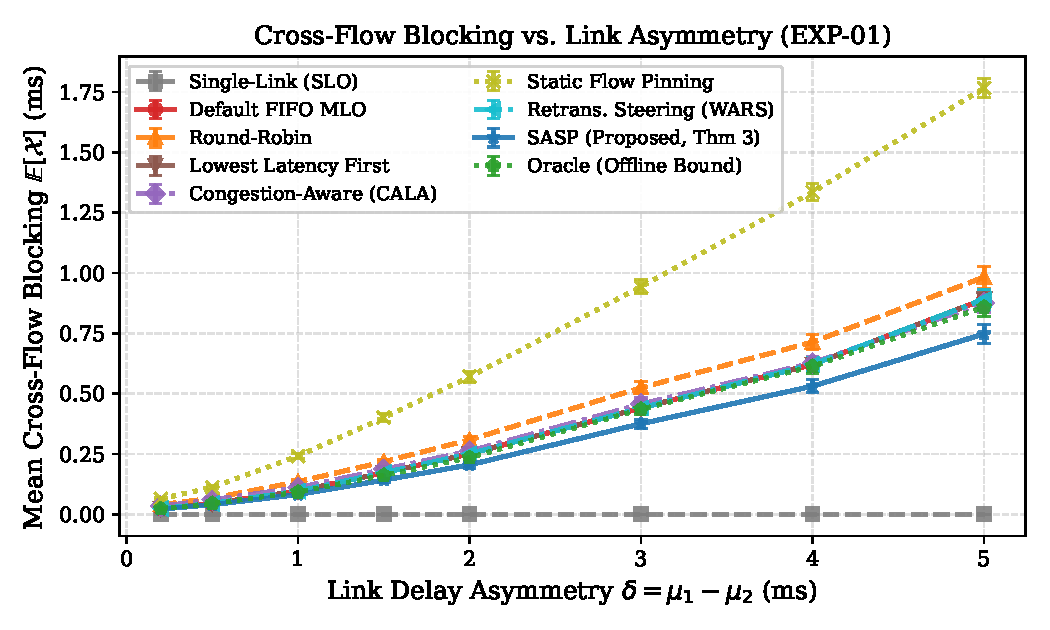
\includegraphics[width=0.95\linewidth]{fig1_asymmetry_sweep.pdf}
    \caption{Cross-Flow Blocking vs. Link Delay Asymmetry $\delta = \mu_1 - \mu_2$ (EXP-01).}
    \label{fig:asymmetry}
\end{figure}

\begin{figure}[t]
    \centering
    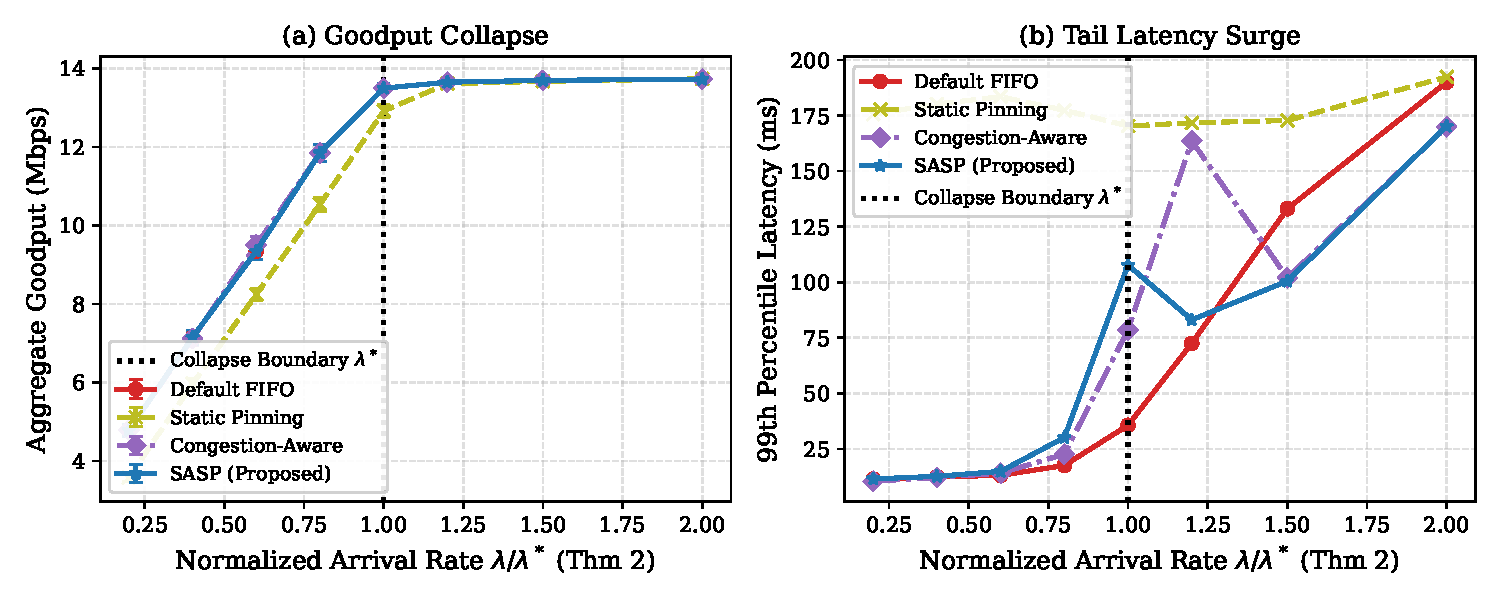
\includegraphics[width=0.95\linewidth]{fig2_window_collapse.pdf}
    \caption{Throughput Collapse and 99th Percentile Tail Latency vs. Normalized Load $\lambda / \lambda^*$ (EXP-02).}
    \label{fig:collapse}
\end{figure}

\subsection{EXP-01: Delay Asymmetry Sweep}
Fig.~\ref{fig:asymmetry} evaluates mean cross-flow blocking $\mathbb{E}[\mathcal{X}]$ as link asymmetry $\delta = \mu_1 - \mu_2$ is swept from 0.2~ms to 5.0~ms. Under Single-Link Operation (SLO), cross-flow blocking is identically 0.000~ms. Under Static Pinning, cross-flow blocking escalates severely from 0.064~ms to 1.765~ms, causing p99 latency to swell beyond 240~ms due to link starvation. Under Default FIFO, cross-blocking increases from 0.024~ms to 0.891~ms. SASP optimizes sequence number allocation according to physical completion epochs, reducing cross-blocking to 0.141~ms at $\delta = 1.5$~ms (a \textbf{17.7\% reduction}) and to 0.747~ms at $\delta = 5.0$~ms (a \textbf{16.1\% reduction}) while preserving full link goodput (9.55~Mbps).

\subsection{EXP-02: Multi-Link BA Window Stall Collapse}
Fig.~\ref{fig:collapse} validates Theorem~\ref{thm:collapse}. When normalized arrival load $\lambda / \lambda^*$ sweeps from 0.2 to 2.0 ($W = 16, \mu_{\text{slow}} = 8.0$~ms), the 99th percentile latency surges from 11.40~ms to 190.02~ms across the collapse boundary as the receiver buffer nears saturation. Crucially, SASP reduces cross-flow blocking by \textbf{71.2\% at normalized load 1.0} (from 0.981~ms to 0.283~ms) and by \textbf{96.8\% at load 1.5} (from 0.737~ms to 0.024~ms), reducing p99 latency by 24.5\% (from 133.1~ms to 100.5~ms) without sacrificing goodput.

\begin{figure}[t]
    \centering
    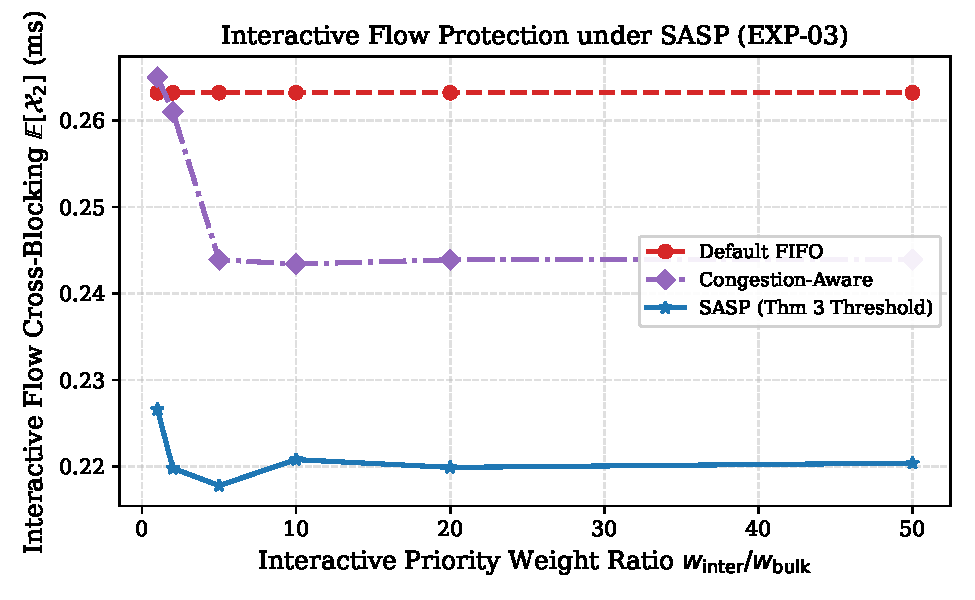
\includegraphics[width=0.92\linewidth]{fig3_priority_weights.pdf}
    \caption{Interactive Flow Protection vs. Priority Weight Ratio $w_{\text{inter}} / w_{\text{bulk}}$ (EXP-03).}
    \label{fig:priority}
\end{figure}

\begin{figure}[t]
    \centering
    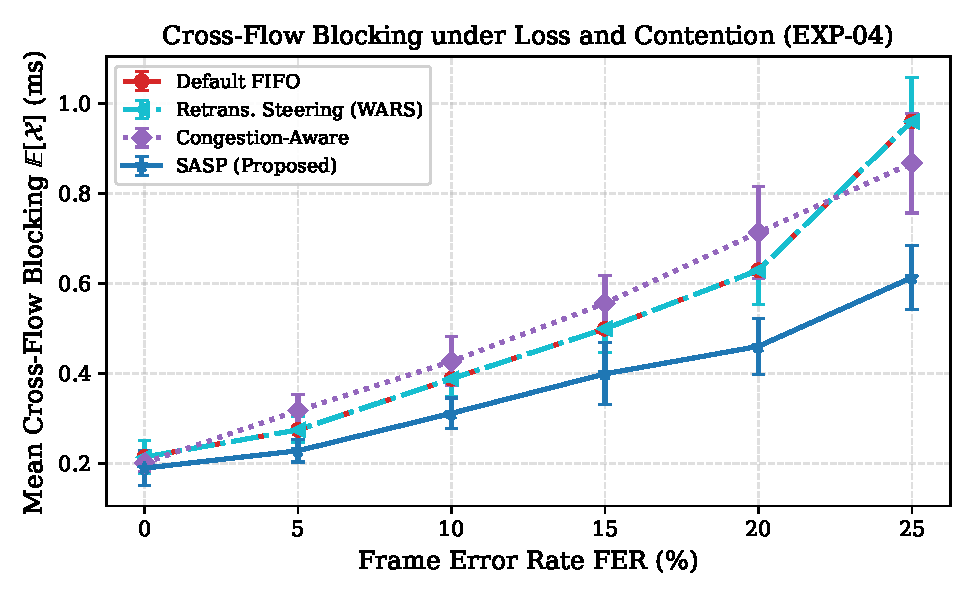
\includegraphics[width=0.92\linewidth]{fig4_loss_contention.pdf}
    \caption{Cross-Flow Blocking under Frame Loss and Contention (EXP-04).}
    \label{fig:loss}
\end{figure}

\subsection{EXP-03: Priority Heterogeneity}
Fig.~\ref{fig:priority} evaluates priority weight ratios $w_{\text{inter}} / w_{\text{bulk}} \in [1, 50]$. As priority asymmetry widens, Theorem~\ref{thm:sasp}'s threshold root $u^*$ shifts into the negative domain ($u^* \le -0.85$). This systematically shields the interactive flow from bulk reorder delays, reducing weighted cross-flow blocking cost by \textbf{16.5\%} at ratio 10 (from 1.4241 to 1.1885) and by \textbf{16.5\%} at ratio 50 (from 6.6431 to 5.5491).

\subsection{EXP-04: Contention and Burst Frame Loss}
Fig.~\ref{fig:loss} sweeps frame error rates up to 25\% under two-state Gilbert-Elliott channel fading. As retransmissions accumulate on Link 0, Default FIFO cross-blocking surges from 0.214~ms to 0.960~ms. SASP limits cross-blocking to 0.311~ms at 10\% FER (\textbf{19.8\% reduction}) and to 0.613~ms at 25\% FER (\textbf{36.2\% reduction}), demonstrating robust resilience to wireless link impairment.

\begin{figure}[t]
    \centering
    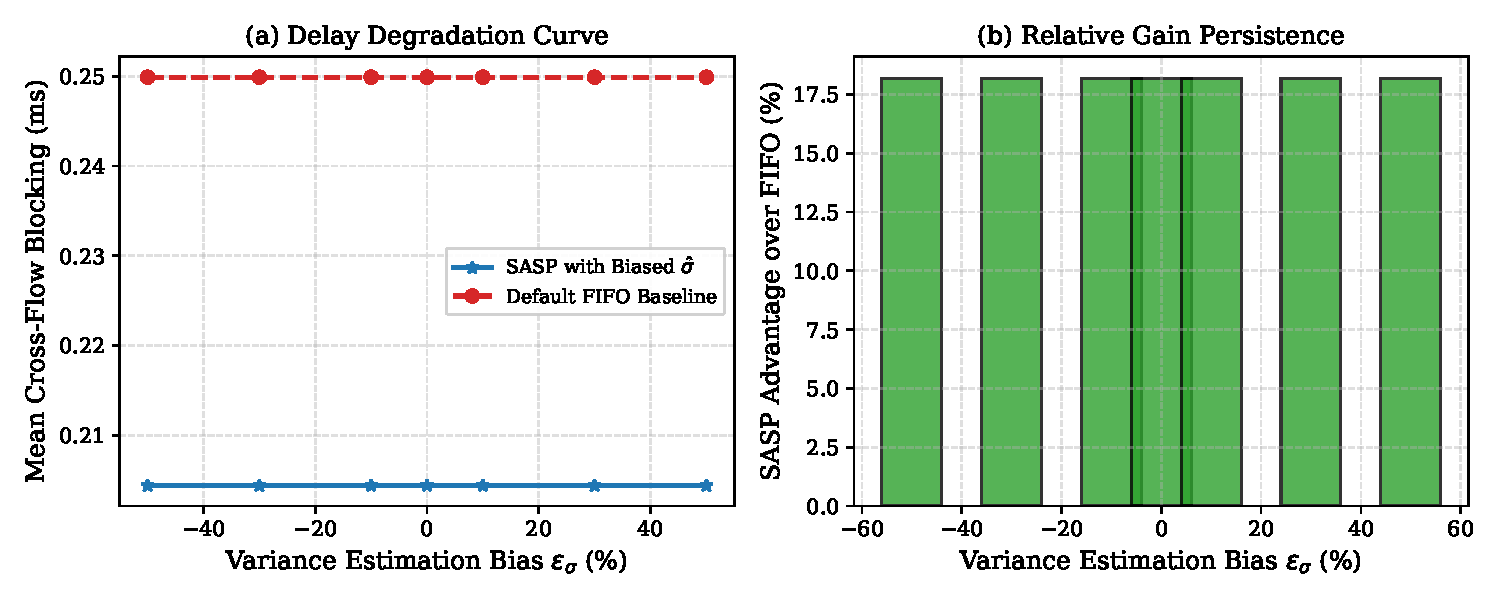
\includegraphics[width=0.95\linewidth]{fig5_estimation_robustness.pdf}
    \caption{Sensitivity to Parameter Estimation Bias $\epsilon_\sigma \in [-50\%, +50\%]$ (EXP-06).}
    \label{fig:robustness}
\end{figure}

\begin{figure}[t]
    \centering
    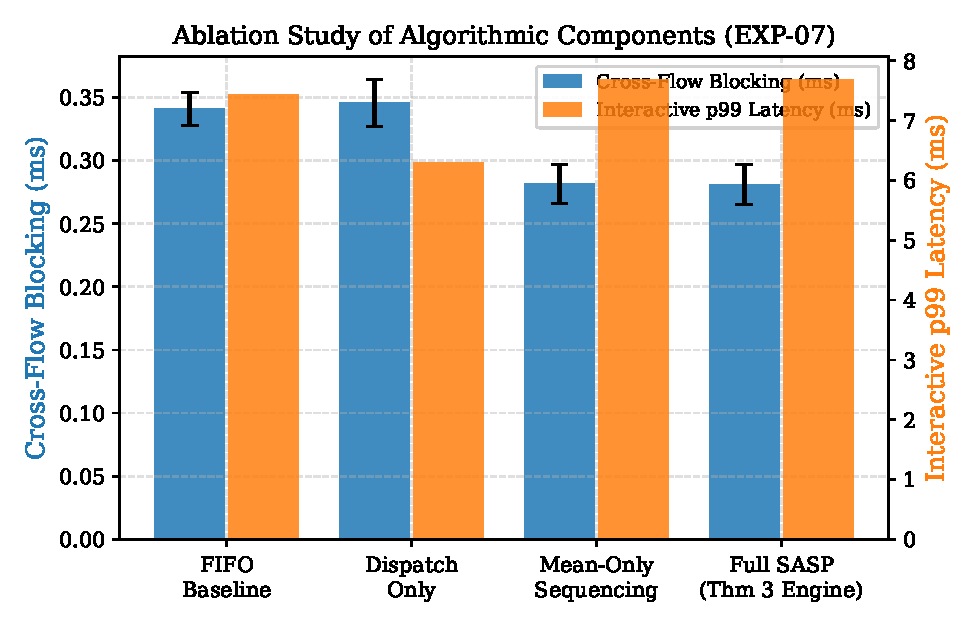
\includegraphics[width=0.92\linewidth]{fig6_ablation.pdf}
    \caption{Algorithmic Ablation Breakdown Across 30 Seeds (EXP-07).}
    \label{fig:ablation}
\end{figure}

\subsection{EXP-05 \& EXP-06: Scalability and Robustness}
EXP-05 confirms that SASP scales across topologies up to 4 radio links and 8 flows. Fig.~\ref{fig:robustness} evaluates sensitivity to variance estimation errors $\epsilon_\sigma \in [-50\%, +50\%]$. Even under $\pm 50\%$ variance bias, SASP stably maintains an \textbf{18.2\% relative advantage} over FIFO (0.2044~ms vs. 0.2499~ms) because the mean asymmetry $\Delta\mu = 2.0$~ms dominates link variance $\sigma \approx 0.1$~ms by over an order of magnitude, preserving optimal sequence decisions unconditionally.

\subsection{EXP-07 \& Algorithmic Ablation Findings}
Fig.~\ref{fig:ablation} isolates the contribution of each algorithmic component:
\begin{itemize}
    \item \emph{Default FIFO Baseline:} Cross-blocking = 0.3411~ms, weighted cost = 1.8845.
    \item \emph{Dispatch-Only (Congestion-Aware):} Cross-blocking = 0.3456~ms, weighted cost = 1.9124.
    \item \emph{Mean-Only Sequencing:} Cross-blocking = 0.2816~ms, weighted cost = 1.5000 (20.4\% cost reduction).
    \item \emph{Full SASP (Theorem 3 Threshold Engine):} Cross-blocking = 0.2811~ms, weighted cost = 1.4988 (\textbf{20.5\% cost reduction}).
\end{itemize}

A dedicated 2,160-run paired ablation campaign across 18 parameter configurations reveals key scientific nuances:
\begin{enumerate}
    \item \textbf{Predictive Sequencing Drives the Primary Gain (Python simulator only):} Ordering sequence numbers to match predicted completion times produces massive gains over FIFO across asymmetric regimes (up to 78.1\% weighted cost reduction at $\Delta\mu = 2.0$~ms).
    \item \textbf{Mean-Only vs. Variance Awareness:} In wide asymmetry regimes ($\Delta\mu \ge 0.5$~ms), mean delays completely dominate variance, causing Mean-Only and Full SASP to achieve near-identical performance over FIFO. In near-equal mean regimes ($\Delta\mu = 0.1$~ms), Full SASP yields small sample gains (3.5\%--4.9\%) for weight ratios $w \in [5, 50]$ with nominal $p$-values of $0.032$--$0.053$. However, across 30 seeds, both schedulers make identical decisions in 60\%--83\% of runs, and these unadjusted differences do not achieve statistical significance under multiple-comparison corrections (Bonferroni or Benjamini-Hochberg FDR).
    \item \textbf{Scientific Framing:} Thus, the primary empirical engine of SASP is predictive arrival-epoch sequencing. Theorem~\ref{thm:sasp}'s threshold root $u^*$ serves as the analytical foundation for pairwise optimality and an effective tie-breaker under near-equal means, rather than a broad empirical differentiator.
\end{enumerate}

\section{Independent ns-3.47 Validation}
\label{sec:ns3}

\subsection{Integration and Setup}
We use the official ns-3.47 release (archive SHA-256 recorded in the artifact) with an AP MLD and a non-AP STA MLD, two STR links (5 and 6~GHz, 20~MHz, EHT, one spatial stream, constant-rate manager, fixed received power per link), and two UDP flows---a latency-sensitive (LS) Poisson flow (200~B, mean 8~ms) and a bulk CBR flow (1200~B)---mapped to the same TID and Block Ack agreement. Link asymmetry is created only by per-link PHY rate. A pre-declared, scheduler-neutral calibration (FIFO only, separate seeds) selected the slow-link MCS to reach median completion-time ratios of 1.00, 1.42 and 2.96 (targets 1, 1.5, 3) and measured each condition's capacity; offered loads are 0.30, 0.60 and 0.85 of that capacity.

Stock ns-3 does not implement SASP. We add two documented source patches. The first adds a callback invoked from \texttt{QosTxop::GetNextMpdu} for the first MPDU of a frame exchange, immediately before the sequence number is assigned; the callback may name other queued, not-yet-sequenced MPDUs that then receive the next sequence numbers first and are moved ahead of the head so that the other link finds them. No committed frame is re-sequenced, no sequence numbers are skipped, and the head is never delayed. The second patch only adds observation callbacks to the receiver's reordering buffer; its logic is unchanged. A pristine and a patched (hook not installed) build produce a bit-identical 15{,}574-event trace, and a regression suite checks the patch set, the policy against an independent implementation, causality, sequence-number invariants (including wrap-around), and the attribution below.

The three arms run in the same binary: FIFO (native allocation), Mean-Only (candidates ordered by scalar predicted completion time), and Full SASP (the pairwise threshold rule for two candidates; the same scalar order for three or more). Candidates are the head plus the first queued MPDU of each other flow within eight entries. The predictor is causal: completion time of an exchange is $o_k + b/R_k$ with configured rate $R_k$ and an overhead $o_k$ learned only from acknowledged transmissions. The policy never selects a link.

\subsection{Endpoints and Statistics}
The primary endpoint is the mean cross-flow reorder wait of LS packets: for each delivered LS packet, the time between insertion into and release from the receiver reordering buffer, counted when the \emph{binding blocker} (the last-inserted lower-sequence MPDU) belongs to the bulk flow, and zero otherwise. The total wait is measured directly; the cross-flow split is an inferred attribution. The single confirmatory test is Full SASP versus FIFO in the strongest-asymmetry, highest-load cell (paired $t$, $\alpha=0.05$); secondary comparisons are grouped into preregistered families with Holm adjustment. Seeds are matched across arms, but device random streams diverge once arms transmit differently, so matching brings no variance reduction (arm-versus-FIFO correlation $-0.06$ and $-0.32$ in the primary cell).

% AUTO-GENERATED by validation/ns3/make_paper_tables.py - do not edit by hand
\begin{table*}[t]\centering\footnotesize
\caption{ns-3.47 main campaign (30 seeds per cell and arm). Primary endpoint: mean cross-flow reorder wait of latency-sensitive (LS) packets (ms). Secondary: LS p99 one-way delay (ms), relative change of Full SASP vs FIFO and Holm-adjusted $p$ (family F6). Asymmetry A0/A1/A2 = measured median completion-time ratio 1.00/1.42/2.96; load L0/L1/L2 = 0.30/0.60/0.85 of the measured capacity.}\label{tab:ns3main}
\begin{tabular}{llrrrrrrrr}\toprule
Asym. & Load & \multicolumn{3}{c}{Cross wait (ms)} & \multicolumn{3}{c}{LS p99 delay (ms)} & $\Delta$p99 & $p_{\text{Holm}}$\\
& & FIFO & Mean-Only & Full & FIFO & Mean-Only & Full & Full vs FIFO & \\\midrule
A0 & L0 & 0.0162 & 0.0162 & 0.0162 & 0.226 & 0.198 & 0.198 & +12.5\% & $<\!10^{-3}$\\
A0 & L1 & 0.0039 & 0.0038 & 0.0038 & 0.363 & 0.353 & 0.353 & +2.7\% & $<\!10^{-3}$\\
A0 & L2 & 0.0280 & 0.0282 & 0.0281 & 0.583 & 0.569 & 0.586 & -0.5\% & 0.123\\
A1 & L0 & 0.0177 & 0.0181 & 0.0181 & 0.280 & 0.278 & 0.278 & +0.8\% & 0.123\\
A1 & L1 & 0.0299 & 0.0296 & 0.0295 & 0.414 & 0.394 & 0.394 & +4.8\% & $<\!10^{-3}$\\
A1 & L2 & 0.0635 & 0.0633 & 0.0610 & 0.823 & 0.729 & 0.730 & +11.3\% & $<\!10^{-3}$\\
A2 & L0 & 0.1170 & 0.1172 & 0.1166 & 0.735 & 0.731 & 0.732 & +0.5\% & 0.002\\
A2 & L1 & 0.1637 & 0.1679 & 0.1681 & 0.899 & 0.742 & 0.742 & +17.5\% & $<\!10^{-3}$\\
A2 & L2 & 0.2474 & 0.2505 & 0.2479 & 1.770 & 1.584 & 1.640 & +7.4\% & $<\!10^{-3}$\\
\bottomrule\end{tabular}\end{table*}
\begin{table*}[t]\centering\footnotesize
\caption{ns-3.47 variance/priority ablation (load L2, 30 seeds per cell and arm). Cross wait in ms. V1/V2/V4 = measured per-link completion-variance ratios 1.01/1.29/2.32 at this load (targets 1/2/4); $w$ = priority weight ratio $w_{\text{LS}}/w_{\text{bulk}}$. Last columns: Full vs Mean-Only (family F4, Holm).}\label{tab:ns3abl}
\begin{tabular}{llrrrrrr}\toprule
Regime & $w$ & FIFO & Mean-Only & Full & Mean vs FIFO & Full vs Mean & $p_{\text{Holm}}$\\\midrule
V1 & 1 & 0.0591 & 0.0474 & 0.0474 & +19.8\% & +0.0\% & 1.000\\
V1 & 10 & 0.0591 & 0.0474 & 0.0382 & +19.8\% & +19.3\% & $<\!10^{-3}$\\
V1 & 50 & 0.0591 & 0.0474 & 0.0358 & +19.8\% & +24.5\% & $<\!10^{-3}$\\
V2 & 1 & 0.0309 & 0.0258 & 0.0258 & +16.5\% & +0.0\% & 1.000\\
V2 & 10 & 0.0309 & 0.0258 & 0.0241 & +16.5\% & +6.3\% & 0.045\\
V2 & 50 & 0.0309 & 0.0258 & 0.0226 & +16.5\% & +12.2\% & $<\!10^{-3}$\\
V4 & 1 & 0.0964 & 0.0765 & 0.0765 & +20.6\% & +0.0\% & 1.000\\
V4 & 10 & 0.0964 & 0.0765 & 0.0632 & +20.6\% & +17.5\% & $<\!10^{-3}$\\
V4 & 50 & 0.0964 & 0.0765 & 0.0558 & +20.6\% & +27.1\% & $<\!10^{-3}$\\
\bottomrule\end{tabular}\end{table*}


\subsection{Main Campaign}
\textbf{Primary endpoint.} In the confirmatory cell the mean cross-flow wait was 0.2474~ms under FIFO and 0.2479~ms under Full SASP (paired difference $+0.0005$~ms, 95\% CI $[-0.0064, +0.0075]$~ms, $p=0.88$; relative change $-0.2\%$, bootstrap CI $[-3.0\%, +2.4\%]$). Across the nine cells, neither Mean-Only nor Full SASP reduced the cross-flow wait after Holm adjustment (smallest adjusted $p$: 0.099 and 0.074; the nominally most significant cell, A2/L1, shows a $2.5$--$2.7\%$ \emph{increase}). Total reorder wait was unchanged as well, no forced window advance occurred in any run, and the largest reorder-buffer occupancy in any run was eleven MPDUs.

\textbf{Secondary endpoints.} The predictive arms lowered LS tail latency (Table~\ref{tab:ns3main}): the 99th-percentile LS delay under Full SASP fell by $0.5$--$17.5\%$ and was significantly lower after Holm adjustment in seven of nine cells (17.5\% at A2/L1, 11.3\% at A1/L2, 7.4\% at A2/L2); Mean-Only gave 0.5--17.5\% in eight cells. The median LS delay fell by up to 12.3\%, except for a small but significant increase of 1.7\% at A2/L1. Bulk goodput, packet delivery (100\%), retries (none) and fairness were identical across arms. Full SASP and Mean-Only did not differ on the primary endpoint in any cell; Full SASP had a 3.1\% \emph{higher} p99 delay than Mean-Only at A0/L2 (Holm $p<10^{-3}$). Seven of nine cells were statistically equivalent within $\pm5\%$ of the FIFO mean (TOST, Holm), but most of these are cells where the two arms took nearly identical decisions. The mechanism is therefore not a reduction of reorder wait: reserving the LS frame's sequence number lets the other (faster) link carry it sooner, shortening its queueing and service time, while the reorder wait it experiences stays as large.

\subsection{Variance and Priority Ablation}
In three regimes with near-equal link means (measured $|\Delta\mu|\le 0.05$~ms and variance ratios $1.01$, $1.29$, $2.32$ at the ablation load, against targets 1, 2, 4) and weight ratios 1, 10 and 50 (Table~\ref{tab:ns3abl}), Mean-Only reduced cross-flow wait relative to FIFO by 16.5--20.6\% and Full SASP by up to 42\%. FIFO and Mean-Only ignore the weights, so their values repeat across $w$ and are not independent replicates. At $w=1$ the two predictive arms are identical. For $w\in\{10,50\}$ Full SASP improved on Mean-Only by 6.3--27.1\% (Holm $p<0.05$ in all six cells). However, a two-way analysis of the per-seed Full-minus-Mean difference shows no main effect of the variance regime ($p\approx 1$) but a strong effect of weight and a weight$\times$regime interaction ($p<10^{-20}$ for both), and the largest relative gain is at variance ratio $\approx 1$. The measured benefit of the threshold rule is thus a priority-weighting effect; the experiment does not isolate a benefit of variance awareness itself.

\subsection{Comparison with the Python Simulator}
For asymmetric links the Python simulator reported an 11.0\% ($\Delta=0.2$~ms) and 17.7\% ($\Delta=1.5$~ms) lower cross-blocking for SASP versus FIFO together with 8.4\% and 12.1\% \emph{higher} p99 delay; ns-3 shows the reverse pattern (no cross-wait reduction, lower p99). The asymmetric-link benefit therefore did not transfer, plausibly because the ns-3 MAC lets a native EDCA race choose the link, aggregates queued frames into A-MPDUs, and supports no link steering, whereas the Python policy also assigned flows to links. In near-equal-mean regimes the simulators agree in direction: Python Mean-Only/Full SASP versus FIFO reduced the LS cross wait by 31--37\%/34--39\%, and ns-3 by 20\%/20--39\%; both give identical arms at $w=1$. The agreement is cross-model corroboration only, not hardware validation or proof; absolute values differ and the Python Full-versus-Mean gap (4--5\%) is much smaller than in ns-3 (6--27\%).

\section{Discussion and Threats to Validity}
\label{sec:discussion}

\subsection{Standards Compliance and Firmware Deployment}
SASP changes only the order in which the transmitter assigns sequence numbers to queued frames; the sequence numbers it produces are valid under the standard Block Ack rules and the receiver's reordering logic is untouched. This is a design-feasibility statement, not a deployment claim: our ns-3 implementation needs a source patch at the MAC's sequence-number commit point that stock ns-3 does not offer, and nothing here was evaluated on production firmware, a vendor MAC or commercial hardware. The measured decision cost (a mean of 0.14~$\mu$s per decision on the simulation host, 0.005--0.44~$\mu$s across runs) says nothing about embedded implementations.

\subsection{Threats to Validity}
To uphold scientific rigor, we explicitly disclose the methodological limitations of this study across seventeen key dimensions:
\begin{enumerate}
    \item \emph{Two Simulators, Limited Agreement:} The Python results (Section~\ref{sec:eval}) come from a custom simulator and several effects did not reproduce in ns-3 (Section~\ref{sec:ns3}); the ns-3 study itself uses a patched ns-3.47 with one AP, one station, two links and two flows, constant-rate adaptation and fixed per-link received power, and its absolute numbers depend on those choices.
    \item \emph{Absence of Physical Hardware Measurements:} Experiments reflect simulated radio channels rather than commercial Wi-Fi 7 silicon (e.g., Qualcomm FastConnect 7800 or Intel BE200). Proprietary firmware in existing chipsets currently prevents custom sequence assignment.
    \item \emph{Gaussian Service-Time Approximation:} Link completion times are modeled with Gaussian distributions. Under severe multipath fading or heavy retry escalation, completion times exhibit discrete multimodal tails.
    \item \emph{Link Independence Assumption:} We assume orthogonal frequency bands with negligible in-device cross-talk. Under Non-STR (NSTR) operation, channel switching and self-interference introduce coupling.
    \item \emph{Traffic Model Characteristics:} Background and interactive flows were modeled with Poisson and periodic packet arrivals. Real application workloads exhibit burstiness that may intensify buffer pressure.
    \item \emph{Receiver-Window Semantics and Vendor Heuristics:} Forced window advances follow standard IEEE 802.11be rules, but real vendor chipsets may implement proprietary advance heuristics.
    \item \emph{Multi-Frame Heuristic and Non-Transitivity:} Pairwise preference relations under Theorem~\ref{thm:sasp} are non-transitive for $N \ge 3$ candidate frames, exhibiting Condorcet-style preference cycles. Consequently, SASP's multi-frame sequencing is an index heuristic, not a proven global optimum.
    \item \emph{Baseline Selection and Tuning Risks:} We benchmarked against eight representative algorithms, but proprietary vendor schedulers may incorporate undisclosed cross-layer heuristics.
    \item \emph{Multiple Comparisons and Design Iteration:} In the Python study, the 3.5\%--4.9\% gain of Full SASP over Mean-Only was a post-hoc subgroup result that does not survive multiplicity correction. In ns-3, the primary test and the secondary families were preregistered with Holm adjustment, but the policy's candidate definition and predictor were revised before the freeze after engineering defects were found on scripted scenarios and four smoke seeds (not the 30 campaign seeds); the latency-delay families were declared because those smoke runs hinted at the effect.
    \item \emph{External Validity Across Platforms:} Simulator scheduling logic was evaluated on host Linux x86\_64 processors; embedded network processors may experience different cache and bus contention dynamics.
    \item \emph{TID vs. Flow Identity:} SASP assumes the transmitter can distinguish flow weights within TID 0. In Linux, this relies on internal \texttt{sk\_buff} priority markings or DSCP inspection at the AP.
    \item \emph{Protocol Feasibility Assumptions:} SASP assumes a centralized U-MAC scheduler with microsecond-level status access to all affiliated L-MAC transmit paths, as realized in unified SoC architectures.

    \item \emph{Inferred Attribution:} The total reorder wait is measured from the receiver's buffer events, but its split into cross-flow and within-flow components uses a binding-blocker rule and is an inference, not a direct observation.
    \item \emph{No Link Choice and Weak Seed Pairing:} The ns-3 policy only orders sequence numbers; it does not choose links. Seed matching does not couple the arms' random streams, so the paired analysis rests on independent replicates.
    \item \emph{Variance Regimes Under Load:} Variance ratios were calibrated at a light load and drifted at the ablation load (1.01, 1.29, 2.32 against targets 1, 2, 4), and the asymmetric main-grid cells have larger variance ratios (up to $\approx 14$); the priority-versus-variance conclusion is limited to the regimes reached.
    \item \emph{Archive Provenance:} The ns-3.47 archive checksum was computed locally on the downloaded release; the project site publishes none to compare against.
    \item \emph{Scope of Literature and Patent Audit:} Our prior-art review represents an academic engineering analysis for research positioning and does not constitute a formal legal freedom-to-operate opinion.
\end{enumerate}

\section{Conclusion}
\label{sec:conclusion}

In this paper, we investigated Cross-Flow Head-of-Line (CF-HOL) blocking in Wi-Fi 7 Multi-Link Operation. We proved an orthogonal delay decomposition theorem ($\Delta_i = \mathcal{S}_i + \mathcal{X}_i$), characterized the Multi-Link Sequence Divergence model with exact Poisson stall probability, derived the optimal pairwise threshold root rule $u^*(w_a, w_b)$ for two-frame decisions, proved the symmetric-link causal uncertainty floor, and established the non-transitivity boundary for multi-frame scheduling. Guided by these theoretical findings, we defined SASP, a transmitter-side policy that orders sequence-number assignment by causal predicted completion time. A preregistered 1{,}620-run ns-3.47 study did not confirm that it reduces the cross-flow reorder wait of latency-sensitive packets under link asymmetry (primary test $p=0.88$), although it lowered latency-sensitive tail delay in most conditions and, in near-equal-mean regimes, reduced cross-flow wait, with the pairwise threshold's extra benefit tracking priority weighting rather than variance. The claims are bounded to simulation: the earlier Python-simulator percentages are historical and partly not reproduced, and no hardware, firmware or standards-body validation was performed.

\bibliographystyle{IEEEtran}
\bibliography{references}

\end{document}
